% The gadgets E, N (Section 3) and A_L, N_L for L=2 (Section 5).
% Layout: top row E -> A_L, bottom row N -> N_L (left column: Section 3, right column: Section 5).
% Every edge is drawn explicitly, one \draw per edge.
% Edge styles: e1, e1p, u1 = weight 1;  e3, u3 = weight 3;  u1, u3 = edges at universal vertices z_i.
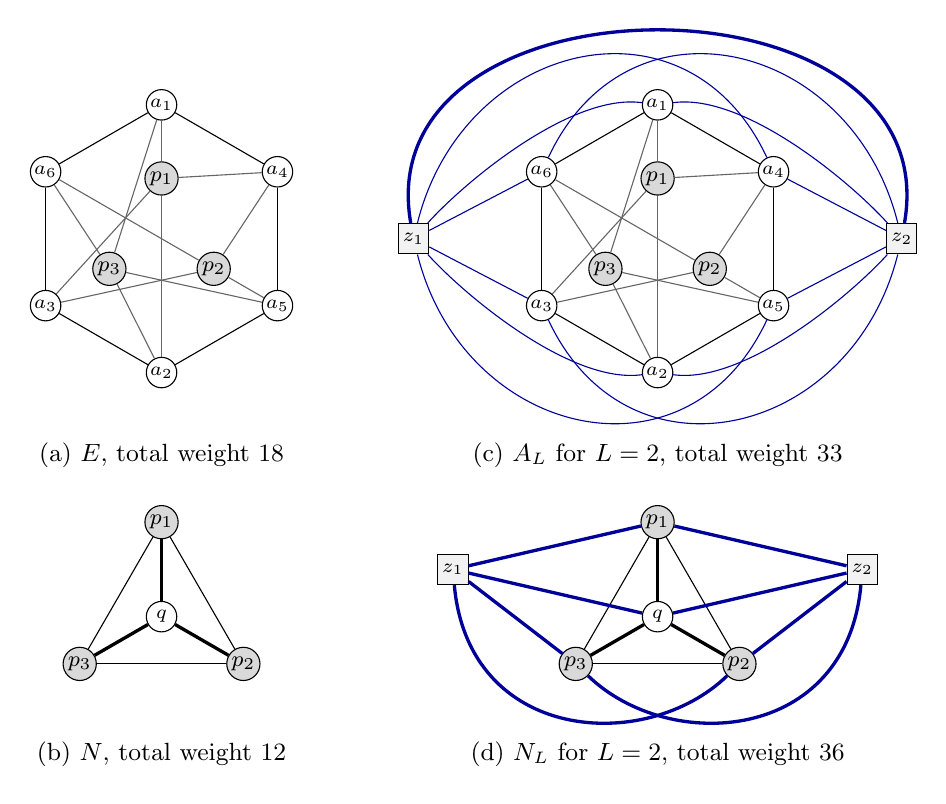
\begin{tikzpicture}[x=1cm,y=1cm,
  prim/.style={circle,draw,fill=black!15,inner sep=0pt,minimum size=12pt,font=\footnotesize},
  aux/.style={circle,draw,fill=white,inner sep=0pt,minimum size=11pt,font=\scriptsize},
  univ/.style={rectangle,draw,fill=black!5,inner sep=0pt,minimum size=11pt,font=\scriptsize},
  e1/.style={line width=0.4pt},
  e1p/.style={line width=0.4pt,black!60},
  e3/.style={line width=1.2pt},
  u1/.style={line width=0.4pt,blue!60!black},
  u3/.style={line width=1.2pt,blue!60!black},
  lab/.style={font=\small}]
% ================================================================== (a) E
\begin{scope}[shift={(0,0)}]
  \node[aux] (aA1) at (90:1.7) {$a_1$};
  \node[aux] (aA4) at (30:1.7) {$a_4$};
  \node[aux] (aA5) at (-30:1.7) {$a_5$};
  \node[aux] (aA2) at (-90:1.7) {$a_2$};
  \node[aux] (aA3) at (-150:1.7) {$a_3$};
  \node[aux] (aA6) at (150:1.7) {$a_6$};
  \node[prim] (pA1) at (90:0.765) {$p_1$};
  \node[prim] (pA2) at (-30:0.765) {$p_2$};
  \node[prim] (pA3) at (210:0.765) {$p_3$};
  % the 6-cycle a1 a4 a5 a2 a3 a6
  \draw[e1] (aA1) -- (aA4);
  \draw[e1] (aA4) -- (aA5);
  \draw[e1] (aA5) -- (aA2);
  \draw[e1] (aA2) -- (aA3);
  \draw[e1] (aA3) -- (aA6);
  \draw[e1] (aA6) -- (aA1);
  % each primary is adjacent to four auxiliary vertices
  \draw[e1p] (pA1) -- (aA1);
  \draw[e1p] (pA1) -- (aA2);
  \draw[e1p] (pA1) -- (aA3);
  \draw[e1p] (pA1) -- (aA4);
  \draw[e1p] (pA2) -- (aA3);
  \draw[e1p] (pA2) -- (aA4);
  \draw[e1p] (pA2) -- (aA5);
  \draw[e1p] (pA2) -- (aA6);
  \draw[e1p] (pA3) -- (aA1);
  \draw[e1p] (pA3) -- (aA2);
  \draw[e1p] (pA3) -- (aA5);
  \draw[e1p] (pA3) -- (aA6);
  \node[lab] at (0,-2.75) {(a) $E$, total weight $18$};
\end{scope}
% ================================================================== (c) A_L, L=2
\begin{scope}[shift={(6.3,0)}]
  \node[aux] (aC1) at (90:1.7) {$a_1$};
  \node[aux] (aC4) at (30:1.7) {$a_4$};
  \node[aux] (aC5) at (-30:1.7) {$a_5$};
  \node[aux] (aC2) at (-90:1.7) {$a_2$};
  \node[aux] (aC3) at (-150:1.7) {$a_3$};
  \node[aux] (aC6) at (150:1.7) {$a_6$};
  \node[prim] (pC1) at (90:0.765) {$p_1$};
  \node[prim] (pC2) at (-30:0.765) {$p_2$};
  \node[prim] (pC3) at (210:0.765) {$p_3$};
  \node[univ] (zC1) at (-3.1,0) {$z_1$};
  \node[univ] (zC2) at (3.1,0) {$z_2$};
  % the gadget E, unchanged
  \draw[e1] (aC1) -- (aC4);
  \draw[e1] (aC4) -- (aC5);
  \draw[e1] (aC5) -- (aC2);
  \draw[e1] (aC2) -- (aC3);
  \draw[e1] (aC3) -- (aC6);
  \draw[e1] (aC6) -- (aC1);
  \draw[e1p] (pC1) -- (aC1);
  \draw[e1p] (pC1) -- (aC2);
  \draw[e1p] (pC1) -- (aC3);
  \draw[e1p] (pC1) -- (aC4);
  \draw[e1p] (pC2) -- (aC3);
  \draw[e1p] (pC2) -- (aC4);
  \draw[e1p] (pC2) -- (aC5);
  \draw[e1p] (pC2) -- (aC6);
  \draw[e1p] (pC3) -- (aC1);
  \draw[e1p] (pC3) -- (aC2);
  \draw[e1p] (pC3) -- (aC5);
  \draw[e1p] (pC3) -- (aC6);
  % z_1, z_2 -- every a_j (weight 1): straight to the nearest two a_j, curved around the cycle to the others
  \draw[u1] (zC1) -- (aC6);
  \draw[u1] (zC1) -- (aC3);
  \draw[u1] (zC2) -- (aC4);
  \draw[u1] (zC2) -- (aC5);
  % (curves are kept out of the bounding box, which would otherwise include their control points;
  %  the \path below adds their true extent)
  \begin{pgfinterruptboundingbox}
  \draw[u1] (zC1) .. controls (-2.43,0.74) and (-1.09,1.85) .. (aC1);
  \draw[u1] (zC1) .. controls (-2.43,-0.74) and (-1.09,-1.85) .. (aC2);
  \draw[u1] (zC1) .. controls (-2.47,2.52) and (0.37,3.21) .. (aC4);
  \draw[u1] (zC1) .. controls (-2.47,-2.52) and (0.37,-3.21) .. (aC5);
  \draw[u1] (zC2) .. controls (2.43,0.74) and (1.09,1.85) .. (aC1);
  \draw[u1] (zC2) .. controls (2.43,-0.74) and (1.09,-1.85) .. (aC2);
  \draw[u1] (zC2) .. controls (2.47,2.52) and (-0.37,3.21) .. (aC6);
  \draw[u1] (zC2) .. controls (2.47,-2.52) and (-0.37,-3.21) .. (aC3);
  % z_1 -- z_2 (weight 3)
  \draw[u3] (zC1) .. controls (-3.71,3.47) and (3.71,3.47) .. (zC2);
  \end{pgfinterruptboundingbox}
  \path (-3.16,-2.36) rectangle (3.16,2.68);
  \node[lab] at (0,-2.75) {(c) $A_L$ for $L=2$, total weight $33$};
\end{scope}
% ================================================================== (b) N
\begin{scope}[shift={(0,-4.8)}]
  \node[prim] (pB1) at (90:1.2) {$p_1$};
  \node[prim] (pB2) at (-30:1.2) {$p_2$};
  \node[prim] (pB3) at (210:1.2) {$p_3$};
  \node[aux] (qB) at (0,0) {$q$};
  \draw[e1] (pB1) -- (pB2);
  \draw[e1] (pB2) -- (pB3);
  \draw[e1] (pB3) -- (pB1);
  \draw[e3] (qB) -- (pB1);
  \draw[e3] (qB) -- (pB2);
  \draw[e3] (qB) -- (pB3);
  \node[lab] at (0,-1.75) {(b) $N$, total weight $12$};
\end{scope}
% ================================================================== (d) N_L, L=2
\begin{scope}[shift={(6.3,-4.8)}]
  \node[prim] (pD1) at (90:1.2) {$p_1$};
  \node[prim] (pD2) at (-30:1.2) {$p_2$};
  \node[prim] (pD3) at (210:1.2) {$p_3$};
  \node[aux] (qD) at (0,0) {$q$};
  % z_i raised above the height of q, so that z_1--q--z_2 is not a straight line (no edge z_1z_2)
  \node[univ] (zD1) at (-2.6,0.6) {$z_1$};
  \node[univ] (zD2) at (2.6,0.6) {$z_2$};
  % the gadget N, unchanged
  \draw[e1] (pD1) -- (pD2);
  \draw[e1] (pD2) -- (pD3);
  \draw[e1] (pD3) -- (pD1);
  \draw[e3] (qD) -- (pD1);
  \draw[e3] (qD) -- (pD2);
  \draw[e3] (qD) -- (pD3);
  % z_i -- q and z_i -- every primary (weight 3); no edge z_1 z_2
  \draw[u3] (zD1) -- (qD);
  \draw[u3] (zD1) -- (pD1);
  \draw[u3] (zD1) -- (pD3);
  \draw[u3] (zD2) -- (qD);
  \draw[u3] (zD2) -- (pD1);
  \draw[u3] (zD2) -- (pD2);
  \begin{pgfinterruptboundingbox}
  \draw[u3] (zD1) .. controls (-2.4,-1.6) and (-0.15,-1.75) .. (pD2);
  \draw[u3] (zD2) .. controls (2.4,-1.6) and (0.15,-1.75) .. (pD3);
  \end{pgfinterruptboundingbox}
  \path (-2.63,-1.38) rectangle (2.63,0);
  \node[lab] at (0,-1.75) {(d) $N_L$ for $L=2$, total weight $36$};
\end{scope}
\end{tikzpicture}
